\section{Rayleigh--Taylor Instability}

\subsection{Physical Mechanism}

The Rayleigh--Taylor instability (RTI) is a hydrodynamic instability that occurs when a dense fluid is accelerated by a lighter one. Under such conditions, perturbations located at the interface between the two fluids may grow over time and generate complex non-linear flow structures.

This instability appears in many physical systems involving strong density gradients and acceleration effects, including astrophysical flows, supernova explosions, atmospheric phenomena, and inertial confinement fusion plasmas. In the context of high-energy-density physics, RTI plays a major role because it can strongly enhance turbulent mixing and degrade the stability of compressible flows.

In inertial confinement fusion configurations, the instability develops during the implosion phase when the dense shell material is accelerated inward by the pressure generated by the ablation of the outer surface. Small imperfections initially present on the capsule surface are amplified during compression and progressively distort the interface.

\begin{figure}[H]
\centering
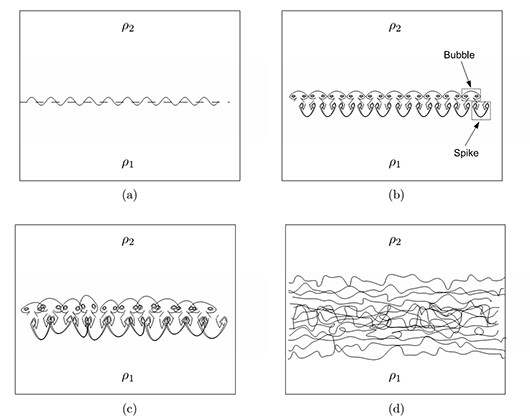
\includegraphics[width=0.55\textwidth]{figures/ch1/rti_sketch.png}
\caption{Illustration of evolution of the Rayleigh--Taylor instability at the interface between two fluids of different densities}
\label{fig:rti_principle}
\end{figure}

As the instability evolves, the interface develops characteristic structures commonly referred to as \textit{bubbles} and \textit{spikes}. The lighter fluid penetrates the denser region through rising bubbles, while the denser fluid penetrates downward through spikes. At later stages, non-linear interactions between structures lead to the formation of increasingly complex flow patterns and eventually to turbulent mixing.

The growth of RTI strongly depends on several physical parameters, including the density contrast between the two fluids, the acceleration field, the viscosity, compressibility effects, and the initial perturbation spectrum. One important dimensionless quantity used to characterize the instability is the Atwood number~\citep[p.~22]{zhou2017rti1}, defined as

\begin{equation}
    A = \frac{\rho_h - \rho_l}{\rho_h + \rho_l}
\end{equation}

where $\rho_h$ and $\rho_l$ denote the densities of the heavy and light fluids respectively. Large Atwood numbers generally correspond to stronger instability growth.


\subsection{Mathematical Origin of the Rayleigh--Taylor Instability}

The Rayleigh--Taylor instability naturally arises from the governing equations of fluid motion when a density stratification is subjected to an acceleration directed from the heavier fluid toward the lighter one. Following the classical development of Kull~\cite{KULL1991197}, the instability can be understood by considering the evolution of small perturbations of an initially hydrostatic equilibrium.

For an incompressible Newtonian fluid, the conservation equations read

\begin{align}
\nabla\cdot\mathbf{u} &= 0,\\
\rho\left(
\frac{\partial\mathbf{u}}{\partial t}
+\mathbf{u}\cdot\nabla\mathbf{u}
\right)
&=
-\nabla p
+\mu\nabla^2\mathbf{u}
+\rho\mathbf{g},
\end{align}

where $\rho$ denotes the density, $\mathbf{u}$ the velocity field, $p$ the pressure and $\mathbf{g}$ the imposed acceleration.

In the absence of motion, the system is in hydrostatic equilibrium,

\begin{equation}
\nabla p_0=\rho\mathbf{g}.
\end{equation}

The stability of this equilibrium depends entirely on the density stratification. When the lighter fluid lies above the heavier one, any perturbation is counteracted by the buoyancy force and the equilibrium is stable. Conversely, when the heavier fluid overlies the lighter one, a small displacement of the interface produces a buoyancy force that amplifies the perturbation rather than restoring it. The hydrostatic equilibrium therefore becomes unstable.

Following the linear stability analysis presented by Kull~\cite{KULL1991197}, the flow variables are decomposed into a base state and infinitesimal perturbations,

\begin{equation}
\mathbf{u}=\mathbf{u}',
\qquad
p=p_0+p',
\qquad
\rho=\rho_0+\rho',
\end{equation}

where only first-order terms are retained. Assuming perturbations of normal-mode form,

\begin{equation}
\exp\left(i\mathbf{k}\cdot\mathbf{x}+\gamma t\right),
\end{equation}

the linearized equations reduce to an eigenvalue problem whose solution provides the perturbation growth rate.

For the ideal case of two incompressible, inviscid fluids separated by a sharp interface and neglecting surface tension, the classical dispersion relation is

\begin{equation}
\gamma^2=Agk,
\end{equation}

The positive sign of $\gamma^2$ demonstrates that disturbances grow exponentially with time,

\begin{equation}
\eta(t)=\eta_0e^{\gamma t},
\end{equation}

revealing that the hydrostatic equilibrium is intrinsically unstable when the acceleration is directed from the heavy fluid toward the light one. This result constitutes the mathematical foundation of the Rayleigh--Taylor instability and explains why small perturbations evolve into the nonlinear structures observed experimentally and numerically.




\subsection{Linear and Non-linear Regimes}

During the early stages of the instability, perturbations remain sufficiently small for linear stability theory to apply. In the incompressible inviscid limit, the perturbation amplitude grows exponentially with growth rate~\citep[p.~23]{zhou2017rti1}

\[
\gamma = \sqrt{A g k},
\]

where $A$ is the Atwood number, $g$ the acceleration, and $k$ the perturbation wavenumber.

As the perturbation amplitude increases, non-linear effects progressively become dominant. Mode coupling mechanisms appear and coherent structures interact across multiple spatial scales. The flow then transitions toward a turbulent mixing regime characterized by strong intermittency and multi-scale dynamics.

% \begin{figure}[htbp]
% \centering
% \fbox{
% \parbox[c][6cm][c]{0.85\textwidth}{
% \centering
% Placeholder for RTI temporal evolution figure
% }}
% \caption{Typical evolution of the Rayleigh--Taylor instability from the linear regime toward turbulent mixing.}
% \label{fig:rti_evolution}
% \end{figure}

This transition from ordered interface perturbations to fully developed turbulent structures constitutes one of the main scientific challenges associated with RTI simulations. The large range of dynamically relevant scales makes accurate numerical prediction particularly difficult.

\subsection{Multi-scale Nature and Turbulence}

One of the main characteristics of the Rayleigh--Taylor instability is its strongly multi-scale behavior. Large coherent structures generated during the non-linear growth phase progressively fragment into smaller vortical structures through turbulent cascades and interface stretching mechanisms.

As turbulence develops, energy is transferred across a wide range of spatial scales. Fine-scale structures emerge near the mixing layer interface and interact continuously with larger coherent motions. This scale coupling significantly complicates both physical analysis and numerical modeling.

\begin{figure}[H]
\centering
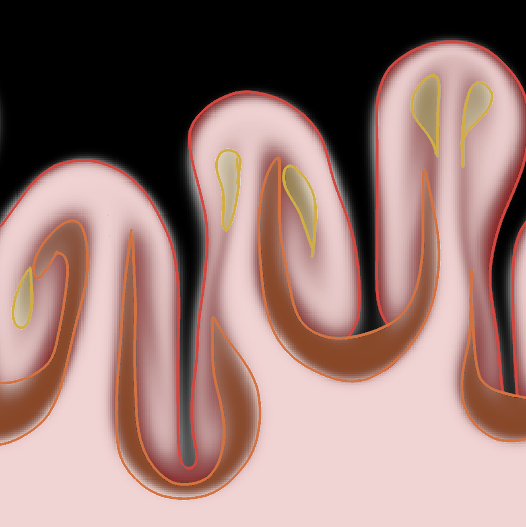
\includegraphics[width=0.30\textwidth]{figures/ch1/RT-MultiScale.png}
\caption{Example of multi-scale structures generated during the turbulent phase of the Rayleigh--Taylor instability}
\label{fig:rti_multiscale}
\end{figure}

The presence of coherent structures, intermittent mixing regions, and localized gradients motivates the use of multi-resolution analysis tools capable of simultaneously capturing both spatial localization and scale-dependent information. This aspect will later motivate the investigation of wavelet-based representations for generative modeling purposes.

